\documentclass[12pt]{article}

\usepackage[utf8]{inputenc}
\usepackage[T1]{fontenc}
\usepackage[polish,provide=*]{babel}
\usepackage{lmodern}
\usepackage{amsmath}
\usepackage{latexsym,amsfonts,amssymb,amsthm,amsmath}
\usepackage{enumitem}
\usepackage{hyperref}
\usepackage{float}
\usepackage{graphicx}
\usepackage{subcaption}
\usepackage{booktabs}
\graphicspath{{./images/}}

\setlength{\parindent}{0in}
\setlength{\oddsidemargin}{0in}
\setlength{\textwidth}{6.5in}
\setlength{\textheight}{8.8in}
\setlength{\topmargin}{0in}
\setlength{\headheight}{18pt}

\title{Pomiar krzywizny soczewki (pierścienie Newtona)}
\author{Kacper Kłos}

\begin{document}
\maketitle

W raporcie opisujemy metodę wyznaczania promienia krzywizny soczewki na podstawie analizy pierścieni Newtona.
Soczewkę umieszczono na płytce szklanej pod mikroskopem, a skalę dopasowano na podstawie papieru milimetrowego położonego na płytce.
Układ oświetlano światłem czerwonym, zielonym i niebieskim.
Po zmierzeniu średnic \(k\)-tych pierścieni dopasowano zależność \(D_k^2(k)\).
Widmo lampy pozwoliło określić długości fal \(\lambda\).
Na tej podstawie obliczono promienie krzywizny dla każdego z kolorów, a średnia ważona dała wynik
\(R = (6{,}613 \pm 0{,}014)\,\mathrm{m}\).

\vspace{1 in}

\section{Wyniki pomiarów}

W tabeli~\ref{tab:rgb_measurements} zestawiono średnice pierścieni (mierzone do środka geometrycznego).

\begin{table}[H]
	\centering
	\begin{tabular}{c|cc|cc|cc}
		\toprule
		Nr & \multicolumn{2}{c|}{\(D_r\,[\mathrm{cm}]\)} & \multicolumn{2}{c|}{\(D_g\,[\mathrm{cm}]\)} & \multicolumn{2}{c}{\(D_b\,[\mathrm{cm}]\)}                            \\
		   & 1                                           & 2                                           & 1                                          & 2      & 1      & 2      \\
		\midrule
		1  & 0{,}33                                      & 0{,}32                                      & 0{,}29                                     & 0{,}30 & 0{,}22 & 0{,}22 \\
		2  & 0{,}44                                      & 0{,}44                                      & 0{,}39                                     & 0{,}40 & 0{,}34 & 0{,}34 \\
		3  & 0{,}52                                      & 0{,}52                                      & 0{,}47                                     & 0{,}48 & 0{,}42 & 0{,}42 \\
		4  & 0{,}60                                      & 0{,}60                                      & 0{,}54                                     & 0{,}54 & 0{,}49 & 0{,}49 \\
		5  & 0{,}67                                      & 0{,}67                                      & 0{,}59                                     & 0{,}60 & 0{,}55 & 0{,}55 \\
		6  & 0{,}74                                      & 0{,}73                                      & 0{,}65                                     & 0{,}66 & 0{,}61 & 0{,}61 \\
		7  & 0{,}78                                      & 0{,}78                                      & 0{,}70                                     & 0{,}70 & 0{,}66 & 0{,}66 \\
		8  & 0{,}84                                      & 0{,}84                                      & 0{,}75                                     & 0{,}76 & 0{,}71 & 0{,}71 \\
		9  & 0{,}88                                      & 0{,}88                                      & 0{,}79                                     & 0{,}79 & 0{,}75 & 0{,}75 \\
		10 & 0{,}92                                      & 0{,}92                                      & 0{,}84                                     & 0{,}84 & 0{,}79 & 0{,}79 \\
		\bottomrule
	\end{tabular}
	\caption{Średnice pierścieni Newtona dla serii pomiarowych 1 i 2. Numery nieparzyste odpowiadają pierścieniom jasnym, parzyste – ciemnym.}
	\label{tab:rgb_measurements}
\end{table}

Niepewność pojedynczego odczytu przyjęto na poziomie \(0{,}01\,\mathrm{cm}\) (dla dwóch pierwszych jasnych pierścieni \(0{,}02\,\mathrm{cm}\) ze względu na ich większą grubość oraz pomiar średnicy przez środek geometryczny).

\subsection{Dopasowanie liniowe}

Wzór teoretyczny podany w~\cite{skrypt} ma postać
\begin{equation}
	D_k^2 = \frac{k \lambda R}{8},
	\label{eq:radius}
\end{equation}
gdzie \(D_k\) – średnica \(k\)-tego pierścienia, \(\lambda\) – długość fali, \(R\) – promień krzywizny.

Średnie wartości z pomiarów (tab.~\ref{tab:rgb_measurements}) dla każdego koloru dopasowujemy do równania \(D_k^2 = a k + b\).

\begin{figure}[H]
	\centering
	\begin{subfigure}{0.3\textwidth}
		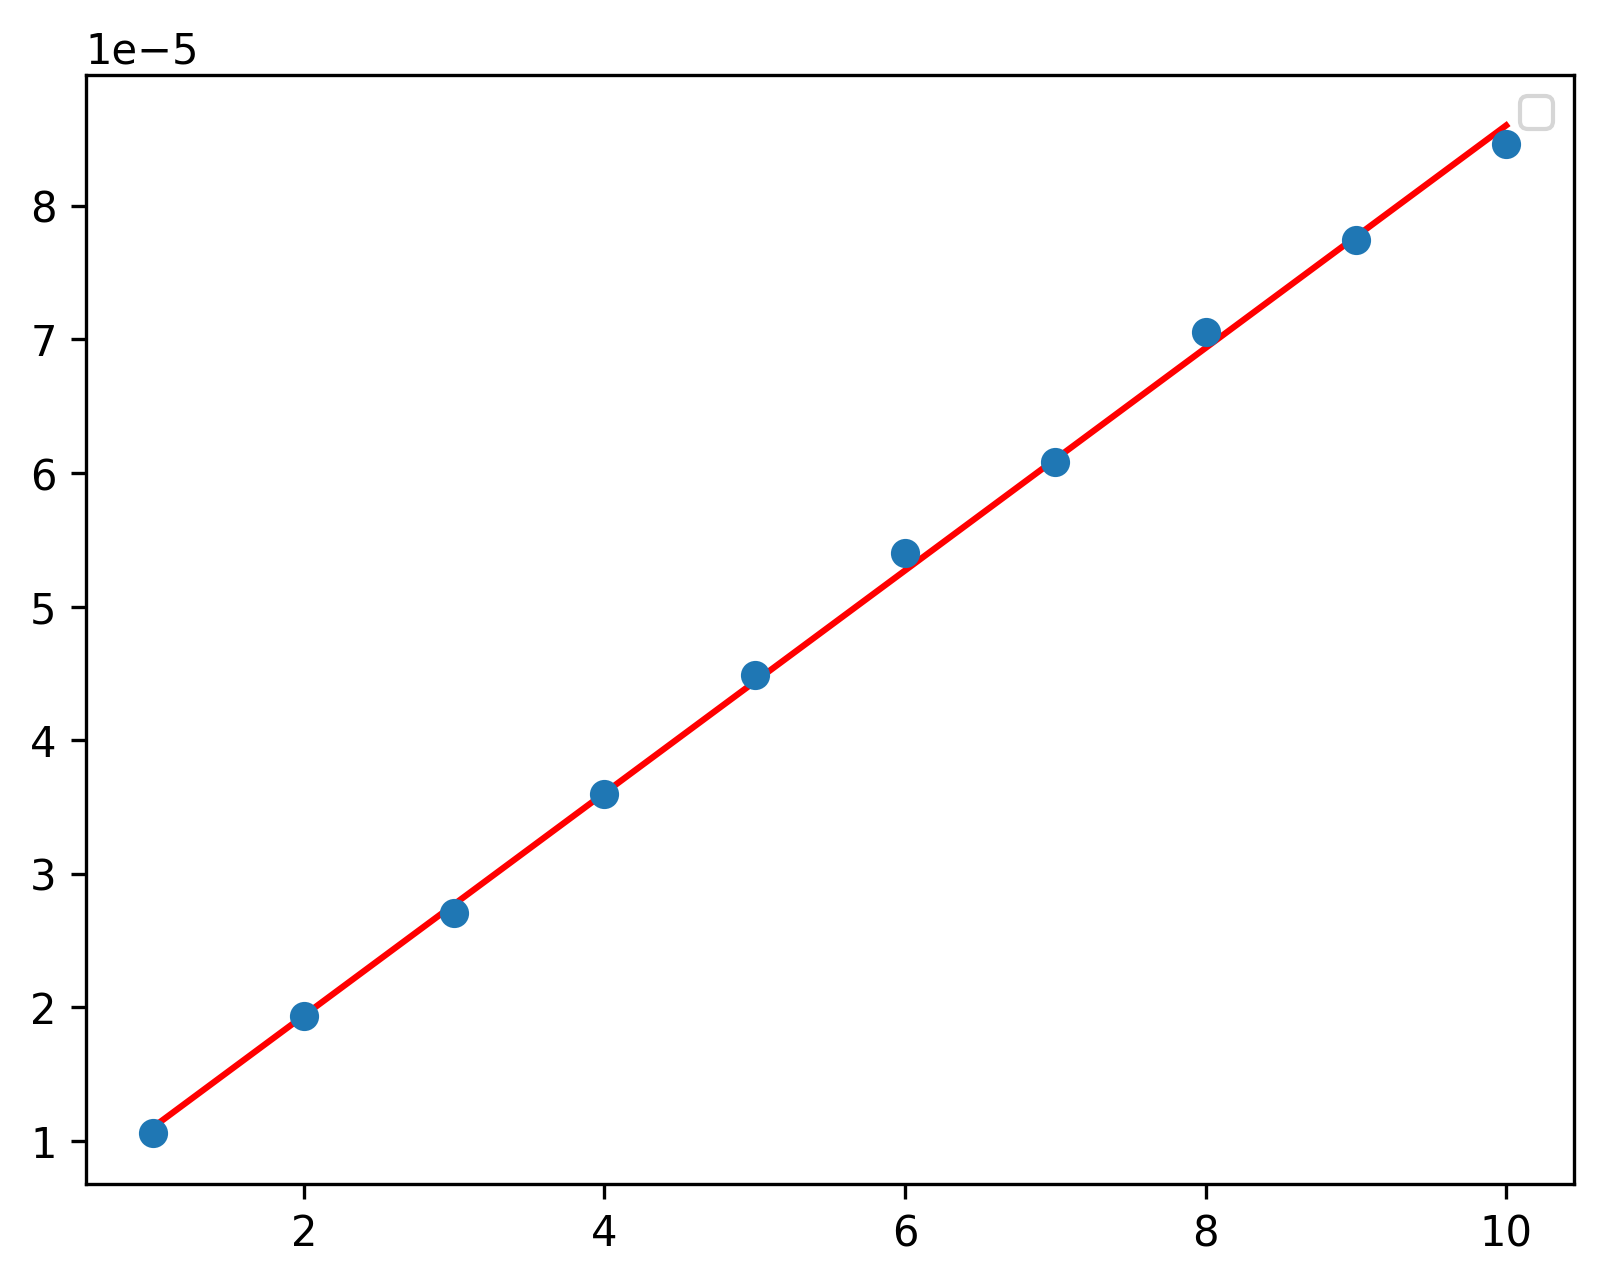
\includegraphics[width=\linewidth]{red}
		\caption{czerwony}
	\end{subfigure}\hfill
	\begin{subfigure}{0.3\textwidth}
		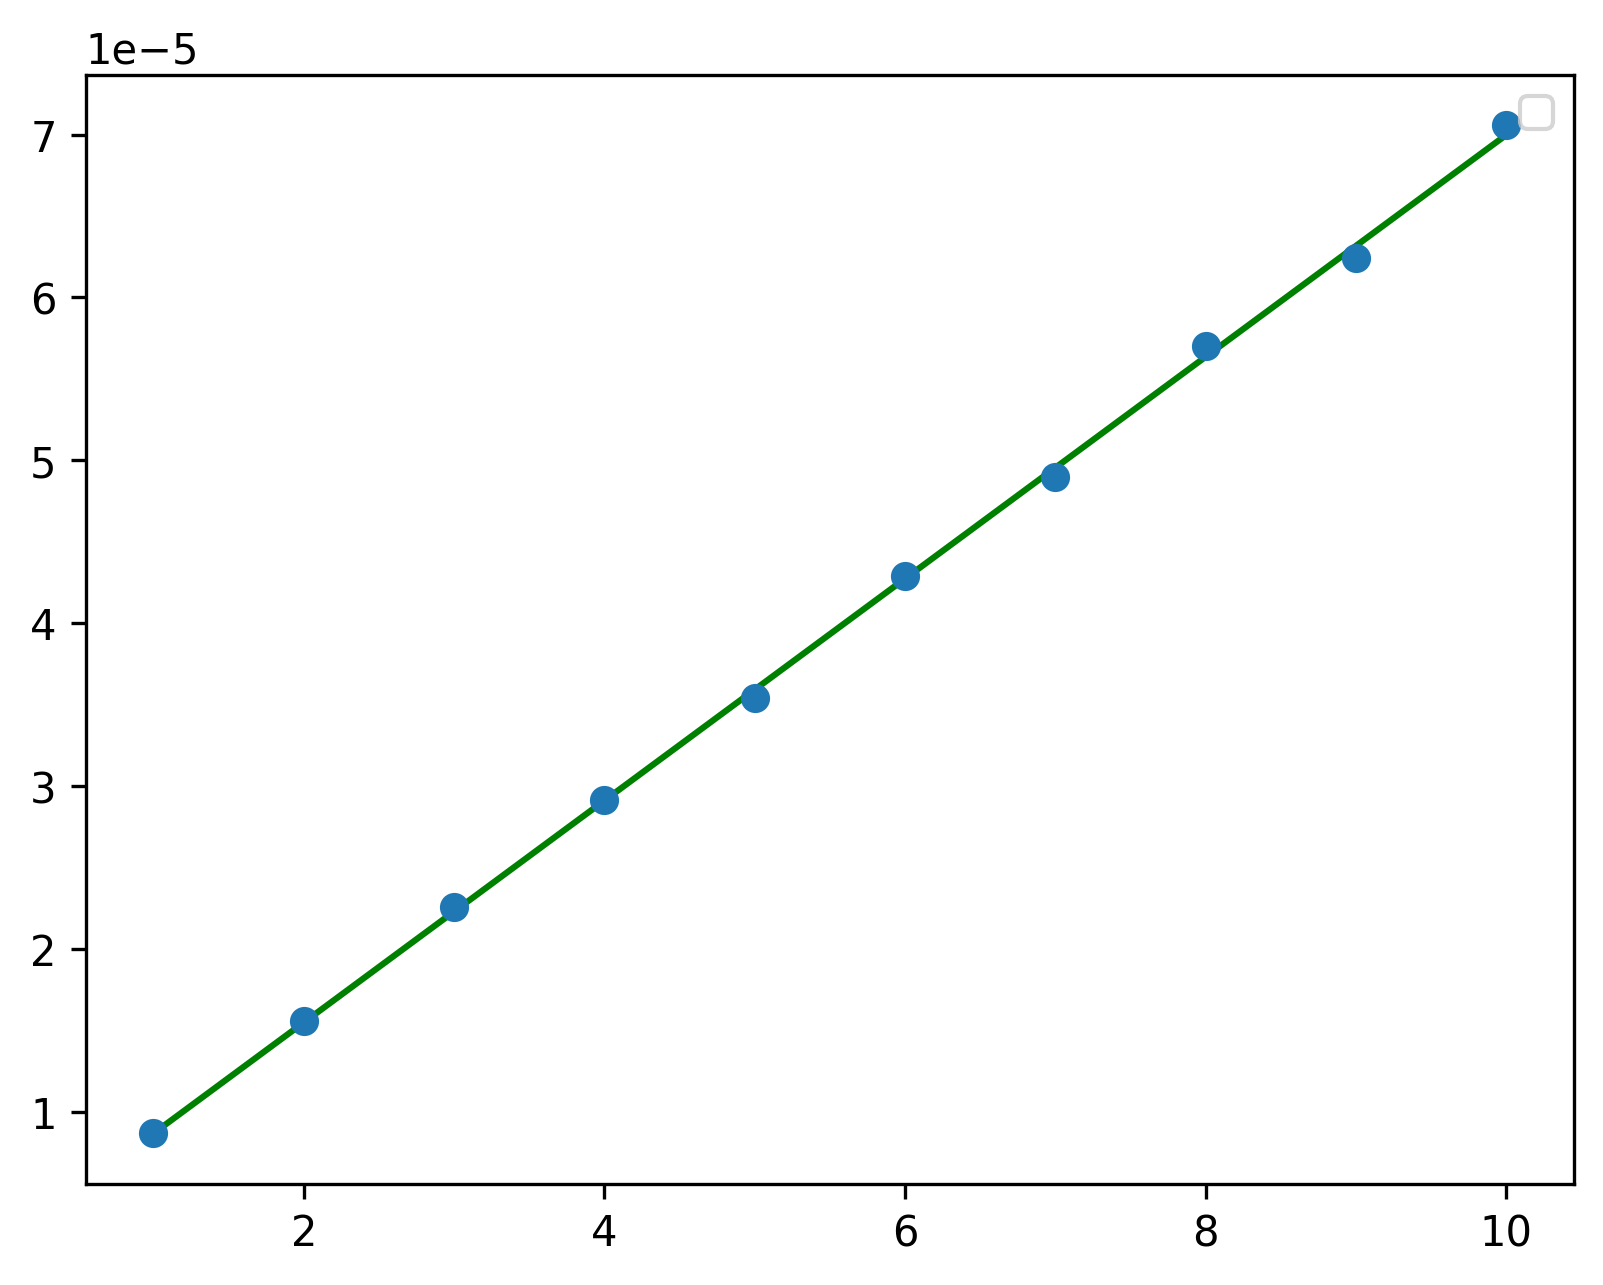
\includegraphics[width=\linewidth]{green}
		\caption{zielony}
	\end{subfigure}\hfill
	\begin{subfigure}{0.3\textwidth}
		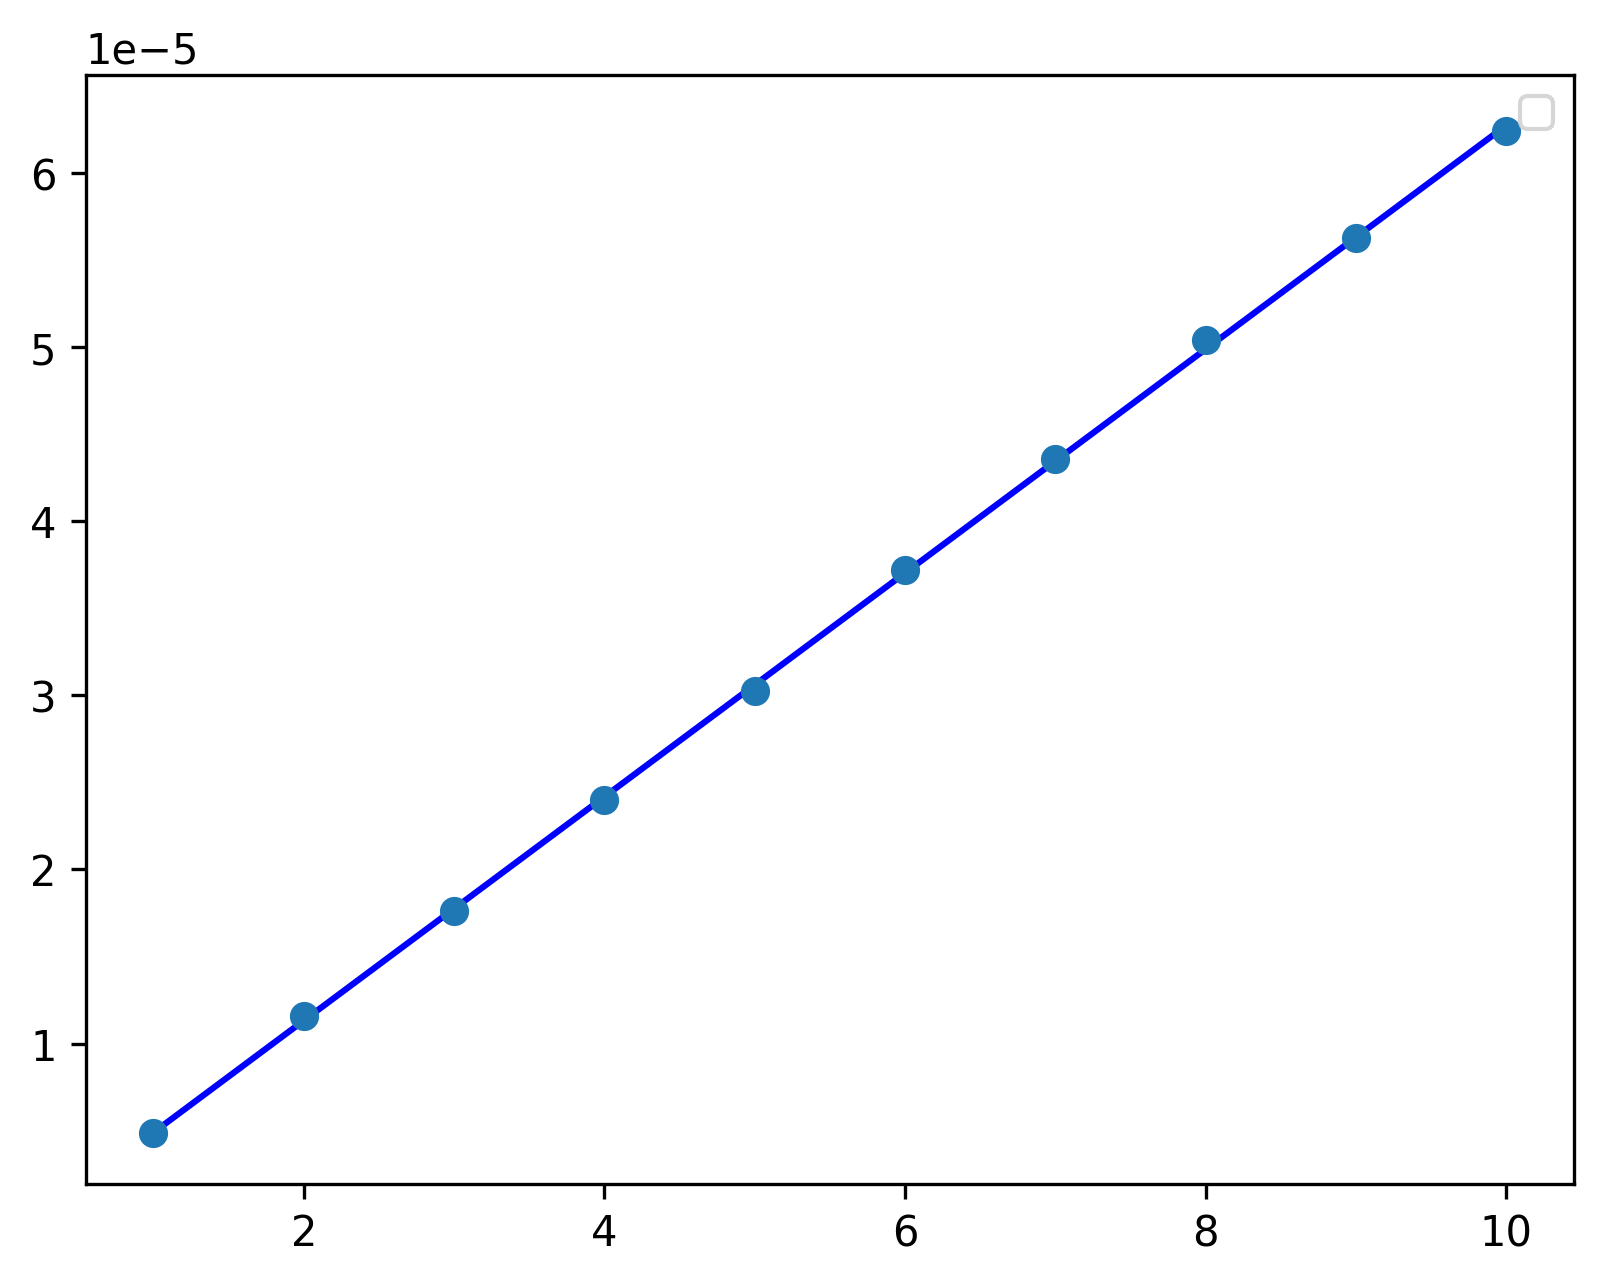
\includegraphics[width=\linewidth]{blue}
		\caption{niebieski}
	\end{subfigure}
	\caption{Dopasowanie liniowe \(D_k^2(k)\) dla trzech barw.}
	\label{fig:line_graphs}
\end{figure}

\begin{table}[H]
	\centering
	\begin{tabular}{c|cc}
		\toprule
		kolor     & \(a\,[10^{-9}]\) & \(b\,[10^{-9}]\) \\
		\midrule
		czerwony  & \(210 \pm 18\)   & \(59 \pm 7\)     \\
		zielony   & \(170 \pm 10\)   & \(49 \pm 4\)     \\
		niebieski & \(161 \pm 8\)    & \(-37 \pm 3\)    \\
		\bottomrule
	\end{tabular}
	\caption{Parametry dopasowania \(D_k^2 = a k + b\).}
	\label{tab:lines_params}
\end{table}

\subsection{Wyznaczenie długości fali}

Długość fali określano z widm lampy: maksimum intensywności oraz punkty o~\(50\%\) tej wartości wyznaczały \(\lambda\) i jej niepewność.
Wykresy widm przedstawiono na rysunkach~\ref{fig:red_wavelength}, \ref{fig:green_wavelength} i~\ref{fig:blue_wavelength}, odpowiadających kolejno światłu czerwonemu, zielonemu i niebieskiemu.

\begin{figure}[H]
	\centering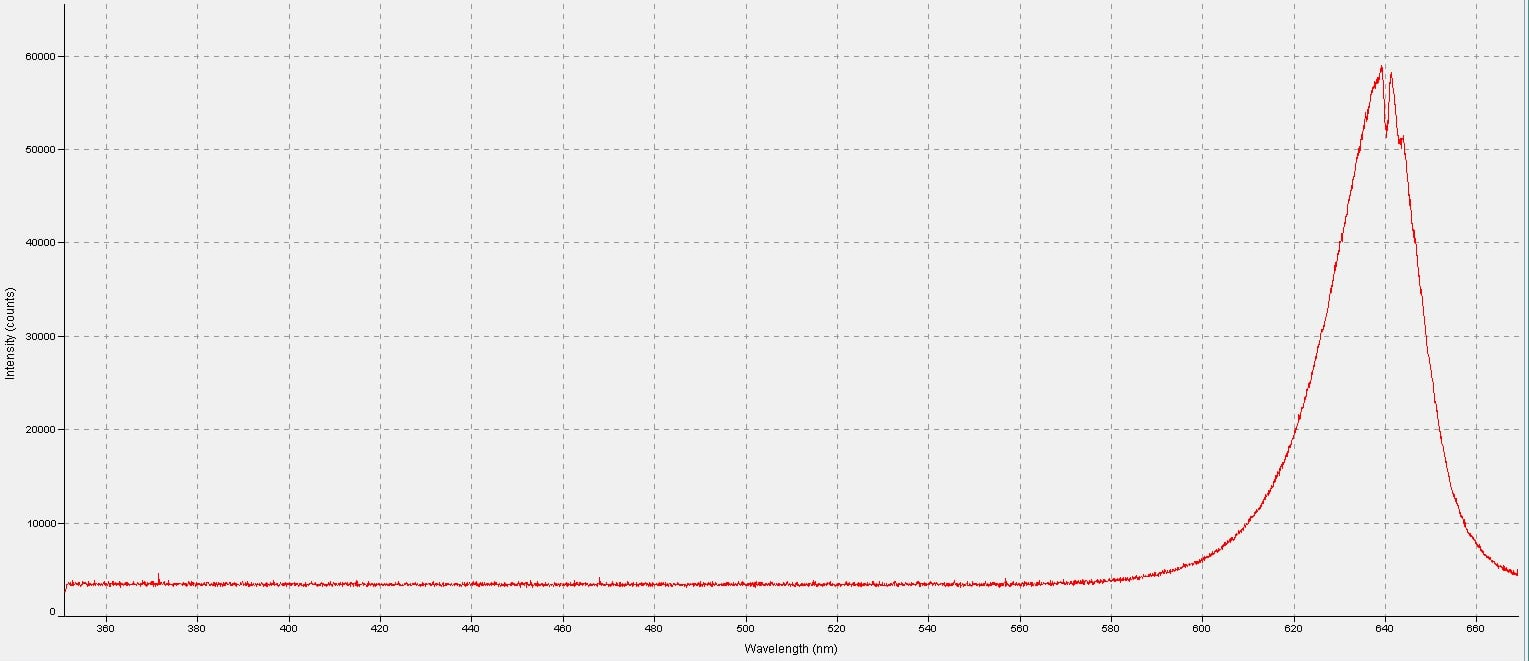
\includegraphics[scale=0.3]{red_wavelength}
	\caption{Widmo światła czerwonego.}
	\label{fig:red_wavelength}
\end{figure}
\begin{figure}[H]
	\centering
	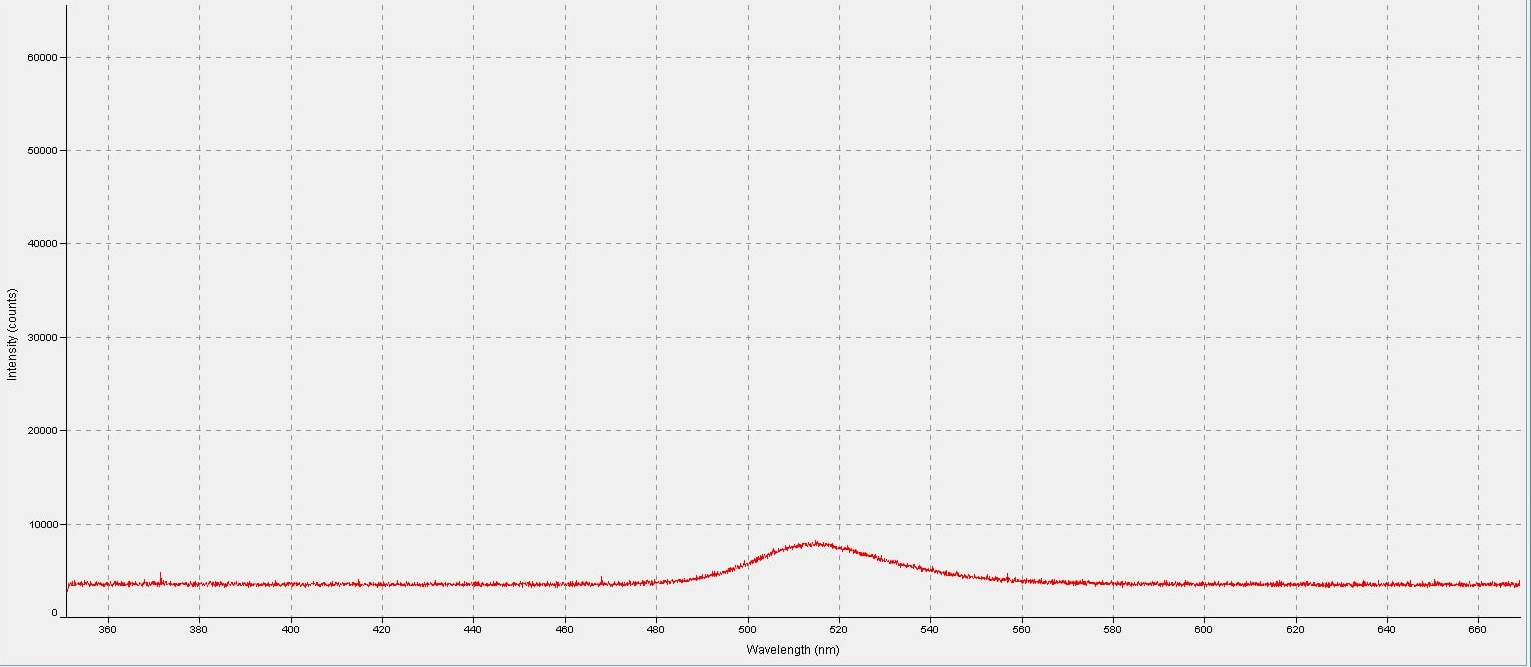
\includegraphics[scale=0.3]{green_wavelength}
	\caption{Widmo światła zielonego.}
	\label{fig:green_wavelength}
\end{figure}
\begin{figure}[H]
	\centering
	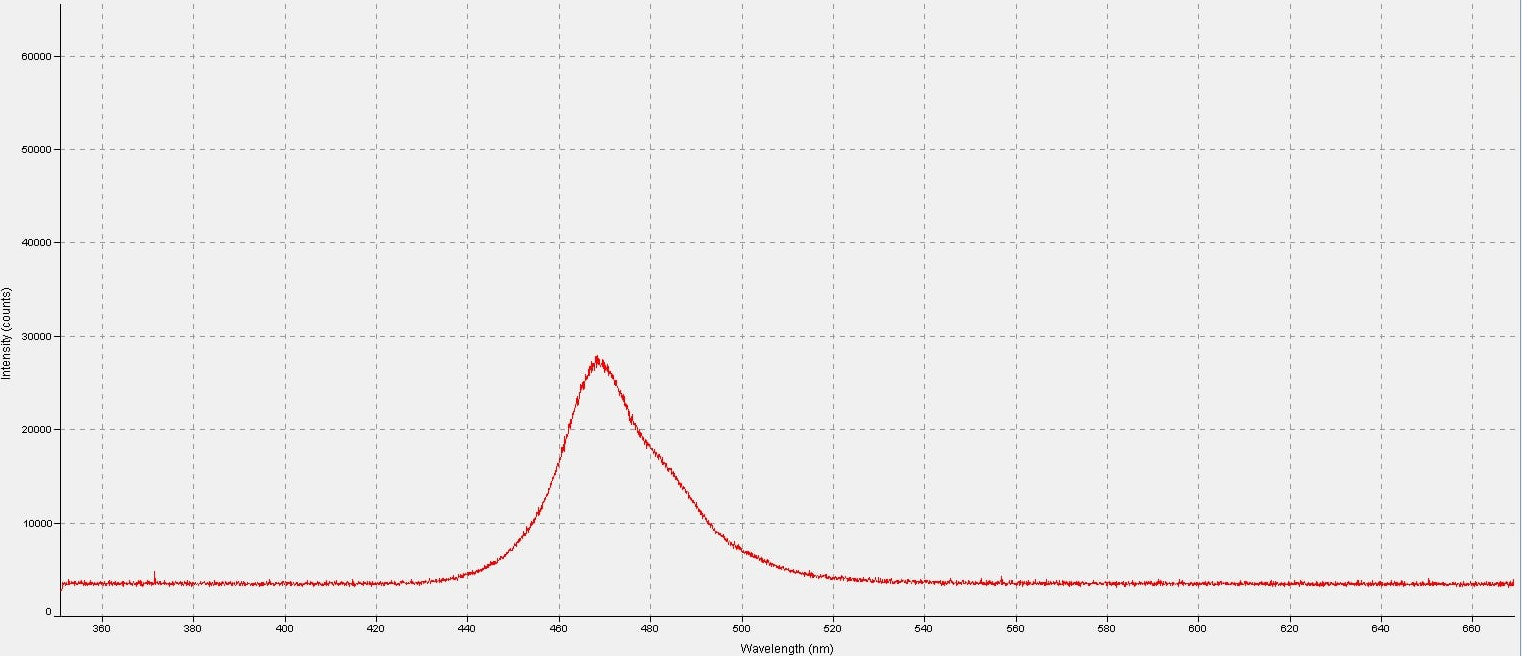
\includegraphics[scale=0.3]{blue_wavelength}
	\caption{Widmo światła niebieskiego.}
	\label{fig:blue_wavelength}
\end{figure}

\begin{table}[H]
	\centering
	\begin{tabular}{c|c}
		\toprule
		kolor     & \(\lambda\,[\mathrm{nm}]\) \\
		\midrule
		czerwony  & \(640 \pm 12\)             \\
		zielony   & \(515 \pm 25\)             \\
		niebieski & \(468 \pm 20\)             \\
		\bottomrule
	\end{tabular}
	\caption{Długości fal użytych świateł.}
	\label{tab:wavelength}
\end{table}

\subsection{Promień krzywizny}

Ze wzorów
\[
	R = 8\,\frac{a}{\lambda}, \qquad
	u(R) = R\sqrt{\left(\frac{u(\lambda)}{\lambda}\right)^2 + \left(\frac{u(a)}{a}\right)^2},
\]
otrzymujemy

\begin{table}[H]
	\centering
	\begin{tabular}{c|c}
		\toprule
		kolor     & \(R\,[\mathrm{m}]\)   \\
		\midrule
		czerwony  & \(6{,}58 \pm 0{,}14\) \\
		zielony   & \(6{,}59 \pm 0{,}40\) \\
		niebieski & \(6{,}86 \pm 0{,}30\) \\
		\bottomrule
	\end{tabular}
	\caption{Promień krzywizny dla poszczególnych barw.}
	\label{tab:radius}
\end{table}

Średnia ważona (na podstawie tabeli~\ref{tab:radius}) daje
\[
	R = 6{,}613 \pm 0{,}014\,\mathrm{m}.
\]

\subsection{Dyskusja niepewności}

Dominującym źródłem niepewności jest dokładność wyznaczenia \(\lambda\).
Choć dopasowanie dla światła czerwonego ma największy błąd współczynnika \(a\), to najmniejsza niepewność \(\lambda\) sprawia, że wynik ten jest najdokładniejszy.
Najbardziej odstaje wartość dla koloru niebieskiego. W szczególności problematyczny jest parametr \(b<0\), co jest sprzeczne z teorią przedstawioną w~\cite{skrypt} i wskazuje na dodatkowy błąd przypadkowy w tej serii pomiarów.
Występuje także błąd systematyczny wynikający z kalibracji skali względem papieru milimetrowego.

\newpage
\begin{thebibliography}{1}

	\bibitem{skrypt}
	\emph{Interferencyjny Pomiar Krzywizny Soczewki (Pierścienie Newtona)}, Uniwersytet Warszawski.

\end{thebibliography}

\end{document}
